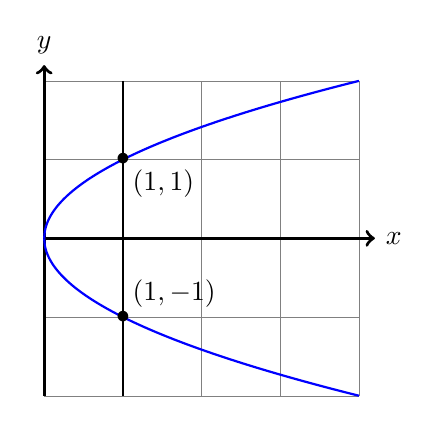
\begin{tikzpicture}[domain=0:4]
  \draw[very thin,color=gray] (0,-2) grid (4,2);

  \draw[very thick,->] (0,0) -- (4.2,0) node[right] {$x$};
  \draw[very thick,->] (0,-2) -- (0,2.2) node[above] {$y$};
  
  \draw [color=blue,thick] plot[smooth,samples=500] (\x,{sqrt(\x)});
  \draw [color=blue,thick] plot[smooth,samples=500] (\x,{-sqrt(\x)});

  \draw [thick] (1,2) -- (1,-2);
  \node at (1,1) {$\bullet$};
  \node [below right] at (1,1) {$(1,1)$};
  
  \node at (1,-1) {$\bullet$};
  \node [above right] at (1,-1) {$(1,-1)$};
\end{tikzpicture}
